%!TEX program = pdflatex
%%%%%%%%%%%%%%%%%%%%%%%%%%%%%%%%%%%%%%%%%
% The Legrand Orange Book
% LaTeX Template
% Version 1.4 (12/4/14)
%
% This template has been downloaded from:
% http://www.LaTeXTemplates.com
%
% Original author:
% Mathias Legrand (legrand.mathias@gmail.com)
%
% License:
% CC BY-NC-SA 3.0 (http://creativecommons.org/licenses/by-nc-sa/3.0/)
%
% Compiling this template:
% This template uses biber for its bibliography and makeindex for its index.
% When you first open the template, compile it from the command line with the 
% commands below to make sure your LaTeX distribution is configured correctly:
%
% 1) pdflatex main
% 2) makeindex main.idx -s StyleInd.ist
% 3) biber main
% 4) pdflatex main x 2
%
% After this, when you wish to update the bibliography/index use the appropriate
% command above and make sure to compile with pdflatex several times 
% afterwards to propagate your changes to the document.
%
% This template also uses a number of packages which may need to be
% updated to the newest versions for the template to compile. It is strongly
% recommended you update your LaTeX distribution if you have any
% compilation errors.
%
% Important note:
% Chapter heading images should have a 2:1 width:height ratio,
% e.g. 920px width and 460px height.
%
%%%%%%%%%%%%%%%%%%%%%%%%%%%%%%%%%%%%%%%%%

%----------------------------------------------------------------------------------------
%	PACKAGES AND OTHER DOCUMENT CONFIGURATIONS
%----------------------------------------------------------------------------------------

\documentclass[11pt,fleqn]{book} % Default font size and left-justified equations

\usepackage[top=3cm,bottom=3cm,left=3.2cm,right=3.2cm,headsep=10pt,a4paper]{geometry} % Page margins

\usepackage[table,xcdraw]{xcolor} % Required for specifying colors by name
\definecolor{verde}{RGB}{51,153,51} % Define the color used for highlighting throughout the book
\definecolor{blue}{rgb}{0.2, 0.2, 0.6}
\definecolor{red}{rgb}{0.8, 0.0, 0.0}
\definecolor{green}{rgb}{0.0, 0.42, 0.24}

% Font Settings
\usepackage{avant} % Use the Avantgarde font for headings
%\usepackage{times} % Use the Times font for headings
\usepackage{mathptmx} % Use the Adobe Times Roman as the default text font together with math symbols from the Sym­bol, Chancery and Com­puter Modern fonts

\usepackage{microtype} % Slightly tweak font spacing for aesthetics
\usepackage[utf8]{inputenc} % Required for including letters with accents
\usepackage[T1]{fontenc} % Use 8-bit encoding that has 256 glyphs
\hyphenation{Mi-nis-té-ri-o}


% Index
\usepackage{calc} % For simpler calculation - used for spacing the index letter headings correctly
\usepackage{makeidx} % Required to make an index
\makeindex % Tells LaTeX to create the files required for indexing
\usepackage{verbatim}

\usepackage[colorinlistoftodos,prependcaption,textsize=tiny,linecolor=red,backgroundcolor=red!25,bordercolor=red]{todonotes}
\usepackage{epigraph}
\renewcommand{\textflush}{flushepinormal}
\setlength{\epigraphwidth}{0.8\textwidth}

\usepackage{nameref}
\usepackage{booktabs}
\usepackage{graphicx}
\usepackage{float}
\usepackage{multirow}


% Bibliography
%\usepackage[backend=biber,style=authoryear,autocite=inline, citestyle=authoryear]{biblatex}
\usepackage[style=abnt]{biblatex}
\addbibresource{bibliography.bib} % BibTeX bibliography file
\defbibheading{bibempty}{}
\renewcommand*{\nameyeardelim}{\addcomma\space}

\newcommand{\VER}[1]{\begingroup\color{red}#1\endgroup}

%----------------------------------------------------------------------------------------

%----------------------------------------------------------------------------------------
%	VARIOUS REQUIRED PACKAGES
%----------------------------------------------------------------------------------------
\usepackage{titlesec} % Allows customization of titles
\usepackage{graphicx} % Required for including pictures
\graphicspath{{Pictures/}} % Specifies the directory where pictures are stored
\usepackage{lipsum} % Inserts dummy text
\usepackage{tikz} % Required for drawing custom shapes
\usepackage[english,brazil]{babel} % English language/hyphenation
\usepackage{enumitem} % Customize lists
\setlist{nolistsep} % Reduce spacing between bullet points and numbered lists
\usepackage{booktabs} % Required for nicer horizontal rules in tables
\usepackage{eso-pic} % Required for specifying an image background in the title page

%----------------------------------------------------------------------------------------
%	MAIN TABLE OF CONTENTS
%----------------------------------------------------------------------------------------
\usepackage{titletoc} % Required for manipulating the table of contents
\contentsmargin{0cm} % Removes the default margin
% Chapter text styling
\titlecontents{chapter}[1.25cm] % Indentation
{\addvspace{20pt}\large\sffamily\bfseries} % Spacing and font options for chapters
{\color{verde!60}\contentslabel[\Large\thecontentslabel]{1.25cm}\color{verde}} % Chapter number
{}  
{\color{verde!60}\normalsize\sffamily\bfseries\;\titlerule*[.5pc]{.}\;\thecontentspage} % Page number
% Section text styling
\titlecontents{section}[1.25cm] % Indentation
{\addvspace{5pt}\sffamily\bfseries} % Spacing and font options for sections
{\contentslabel[\thecontentslabel]{1.25cm}} % Section number
{}
{\sffamily\hfill\color{black}\thecontentspage} % Page number
[]
% Subsection text styling
\titlecontents{subsection}[1.25cm] % Indentation
{\addvspace{15pt}\sffamily\small} % Spacing and font options for subsections
{\contentslabel[\thecontentslabel]{1.25cm}} % Subsection number
{}
{\sffamily\;\titlerule*[.5pc]{.}\;\thecontentspage} % Page number
[] 
%----------------------------------------------------------------------------------------
%	MINI TABLE OF CONTENTS IN CHAPTER HEADS
%----------------------------------------------------------------------------------------
% Section text styling
\titlecontents{lsection}[.05em] % Indendating
{\footnotesize\sffamily} % Font settings
{}
{}
{}
% Subsection text styling
\titlecontents{lsubsection}[.5em] % Indentation
{\normalfont\footnotesize\sffamily} % Font settings
{}
{}
{}
%----------------------------------------------------------------------------------------
%	PAGE HEADERS
%----------------------------------------------------------------------------------------
\usepackage{fancyhdr} % Required for header and footer configuration
\pagestyle{fancy}
\renewcommand{\chaptermark}[1]{\markboth{\sffamily\normalsize\bfseries\chaptername\ \thechapter.\ #1}{}} % Chapter text font settings
\renewcommand{\sectionmark}[1]{\markright{\sffamily\normalsize\thesection\hspace{2pt}#1}{}} % Section text font settings
\fancyhf{} \fancyhead[LE,RO]{\sffamily\normalsize\thepage} % Font setting for the page number in the header
%\fancyhead[LO]{\rightmark} % Print the nearest section name on the left side of odd pages
\fancyhead[RE]{\leftmark} % Print the current chapter name on the right side of even pages
\renewcommand{\headrulewidth}{0.5pt} % Width of the rule under the header
\addtolength{\headheight}{2.5pt} % Increase the spacing around the header slightly
\renewcommand{\footrulewidth}{0pt} % Removes the rule in the footer
\fancypagestyle{plain}{\fancyhead{}\renewcommand{\headrulewidth}{0pt}} % Style for when a plain pagestyle is specified
% Removes the header from odd empty pages at the end of chapters
\makeatletter
\renewcommand{\cleardoublepage}{
\clearpage\ifodd\c@page\else
\hbox{}
\vspace*{\fill}
\thispagestyle{empty}
\newpage
\fi}
%----------------------------------------------------------------------------------------
%	THEOREM STYLES
%----------------------------------------------------------------------------------------
\usepackage{amsmath,amsfonts,amssymb,amsthm} % For math equations, theorems, symbols, etc
\newcommand{\intoo}[2]{\mathopen{]}#1\,;#2\mathclose{[}}
\newcommand{\ud}{\mathop{\mathrm{{}d}}\mathopen{}}
\newcommand{\intff}[2]{\mathopen{[}#1\,;#2\mathclose{]}}
\newtheorem{notation}{Notation}[chapter]
%----------------------------------------------------------------------------------------
%	DEFINITION OF COLORED BOXES
%----------------------------------------------------------------------------------------
\RequirePackage[framemethod=default]{mdframed} % Required for creating the theorem, definition, exercise and corollary boxes
%----------------------------------------------------------------------------------------
%	REMARK ENVIRONMENT
%----------------------------------------------------------------------------------------
\newenvironment{remark}{\par\vspace{10pt}\small % Vertical white space above the remark and smaller font size
\begin{list}{}{
\leftmargin=35pt % Indentation on the left
\rightmargin=25pt}\item\ignorespaces % Indentation on the right
\makebox[-2.5pt]{\begin{tikzpicture}[overlay]
\node[draw=verde!60,line width=1pt,circle,fill=verde!25,font=\sffamily\bfseries,inner sep=2pt,outer sep=0pt] at (-15pt,0pt){\textcolor{verde}{R}};\end{tikzpicture}} % Orange R in a circle
\advance\baselineskip -1pt}{\end{list}\vskip5pt} % Tighter line spacing and white space after remark
%----------------------------------------------------------------------------------------
%	SECTION NUMBERING IN THE MARGIN
%----------------------------------------------------------------------------------------
\makeatletter
\renewcommand{\@seccntformat}[1]{\llap{\textcolor{verde}{\csname the#1\endcsname}\hspace{1em}}}                    
\renewcommand{\section}{\@startsection{section}{1}{\z@}
{-4ex \@plus -1ex \@minus -.4ex}
{1ex \@plus.2ex }
{\normalfont\large\sffamily\bfseries}}
\renewcommand{\subsection}{\@startsection {subsection}{2}{\z@}
{-3ex \@plus -0.1ex \@minus -.4ex}
{0.5ex \@plus.2ex }
{\normalfont\sffamily\bfseries}}
\renewcommand{\subsubsection}{\@startsection {subsubsection}{3}{\z@}
{-2ex \@plus -0.1ex \@minus -.2ex}
{.2ex \@plus.2ex }
{\normalfont\small\sffamily\bfseries}}                        
\renewcommand\paragraph{\@startsection{paragraph}{4}{\z@}
{-2ex \@plus-.2ex \@minus .2ex}
{.1ex}
{\normalfont\small\sffamily\bfseries}}
%----------------------------------------------------------------------------------------
%	HYPERLINKS IN THE DOCUMENTS
%----------------------------------------------------------------------------------------
% For an unclear reason, the package should be loaded now and not later
\usepackage{hyperref}
\hypersetup{hidelinks,backref=true,pagebackref=true,hyperindex=true,colorlinks=false,breaklinks=true,
	urlcolor=verde,bookmarks=true,bookmarksopen=false,pdftitle={Title},pdfauthor={Author}}
%----------------------------------------------------------------------------------------
%	CHAPTER HEADINGS
%----------------------------------------------------------------------------------------
% The set-up below should be (sadly) manually adapted to the overall margin page septup controlled by the geometry package loaded in the main.tex document. It is possible to implement below the dimensions used in the goemetry package (top,bottom,left,right)... TO BE DONE
\newcommand{\thechapterimage}{}
\newcommand{\chapterimage}[1]{\renewcommand{\thechapterimage}{#1}}
% Numbered chapters with mini tableofcontents
\def\thechapter{\arabic{chapter}}
\def\@makechapterhead#1{
\thispagestyle{empty}
{\centering \normalfont\sffamily
\ifnum \c@secnumdepth >\m@ne
\if@mainmatter
\startcontents
\begin{tikzpicture}[remember picture,overlay]
\node at (current page.north west)
{\begin{tikzpicture}[remember picture,overlay]
\node[rounded corners=5pt,anchor=north west,inner sep=0pt] at (0,0) {\includegraphics[width=\paperwidth]{\thechapterimage}};
%%%%%%%%%%%%%%%%%%%%%%%%%%%%%%%%%%%%%%%%%%%%%%%%%%%%%%%%%%%%%%%%%%%%%%%%%%%%%%%%%%%%%
%Tamanho do mini table of contents
\fill[color=verde!10!white,opacity=.6] (.5cm,0) rectangle (9.9cm,-13cm);
%Conteúdo do mini table of contents 
\node[rounded corners=10pt,anchor=north west] at (1.1cm,.35cm) {\parbox[t][10cm][t]{10cm}{\huge\bfseries\flushleft \printcontents{l}{1}{\setcounter{tocdepth}{2}}}};
%Titulo do capitulo
\draw[anchor=west] (10cm,-10cm) node [rounded corners=5pt,fill=verde!10!white,text opacity=1,draw=verde,draw opacity=1,line width=1.5pt,fill opacity=.6,inner sep=12pt]{\huge\sffamily\bfseries\textcolor{black}{\thechapter. #1\strut\makebox[20cm]{}}};
%%%%%%%%%%%%%%%%%%%%%%%%%%%%%%%%%%%%%%%%%%%%%%%%%%%%%%%%%%%%%%%%%%%%%%%%%%%%%%%%%%%%%
\end{tikzpicture}};
\end{tikzpicture}}
\par\vspace*{230\p@}
\fi
\fi}
% Unnumbered chapters without mini tableofcontents (could be added though) 
\def\@makeschapterhead#1{
\thispagestyle{empty}
{\centering \normalfont\sffamily
\ifnum \c@secnumdepth >\m@ne
\if@mainmatter
\begin{tikzpicture}[remember picture,overlay]
\node at (current page.north west)
{\begin{tikzpicture}[remember picture,overlay]
\node[anchor=north west,inner sep=0pt] at (0,0) {\includegraphics[width=\paperwidth]{\thechapterimage}};
\draw[anchor=west] (2cm,-9cm) node [rounded corners=5pt,fill=verde!10!white,fill opacity=.6,inner sep=12pt,text opacity=1,draw=verde,draw opacity=1,line width=1.5pt]{\huge\sffamily\bfseries\textcolor{black}{#1\strut\makebox[22cm]{}}};
\end{tikzpicture}};
\end{tikzpicture}}
\par\vspace*{230\p@}
\fi
\fi
}
\makeatother % Insert the commands.tex file which contains the majority of the structure behind the template

\begin{document}

\let\cleardoublepage\clearpage

\renewcommand{\chaptername}{Capítulo}
\renewcommand{\figurename}{Fig.}

%----------------------------------------------------------------------------------------
%	TITLE PAGE
%----------------------------------------------------------------------------------------
\begingroup
	\thispagestyle{empty}
	
	\AddToShipoutPicture*{\put(0,0){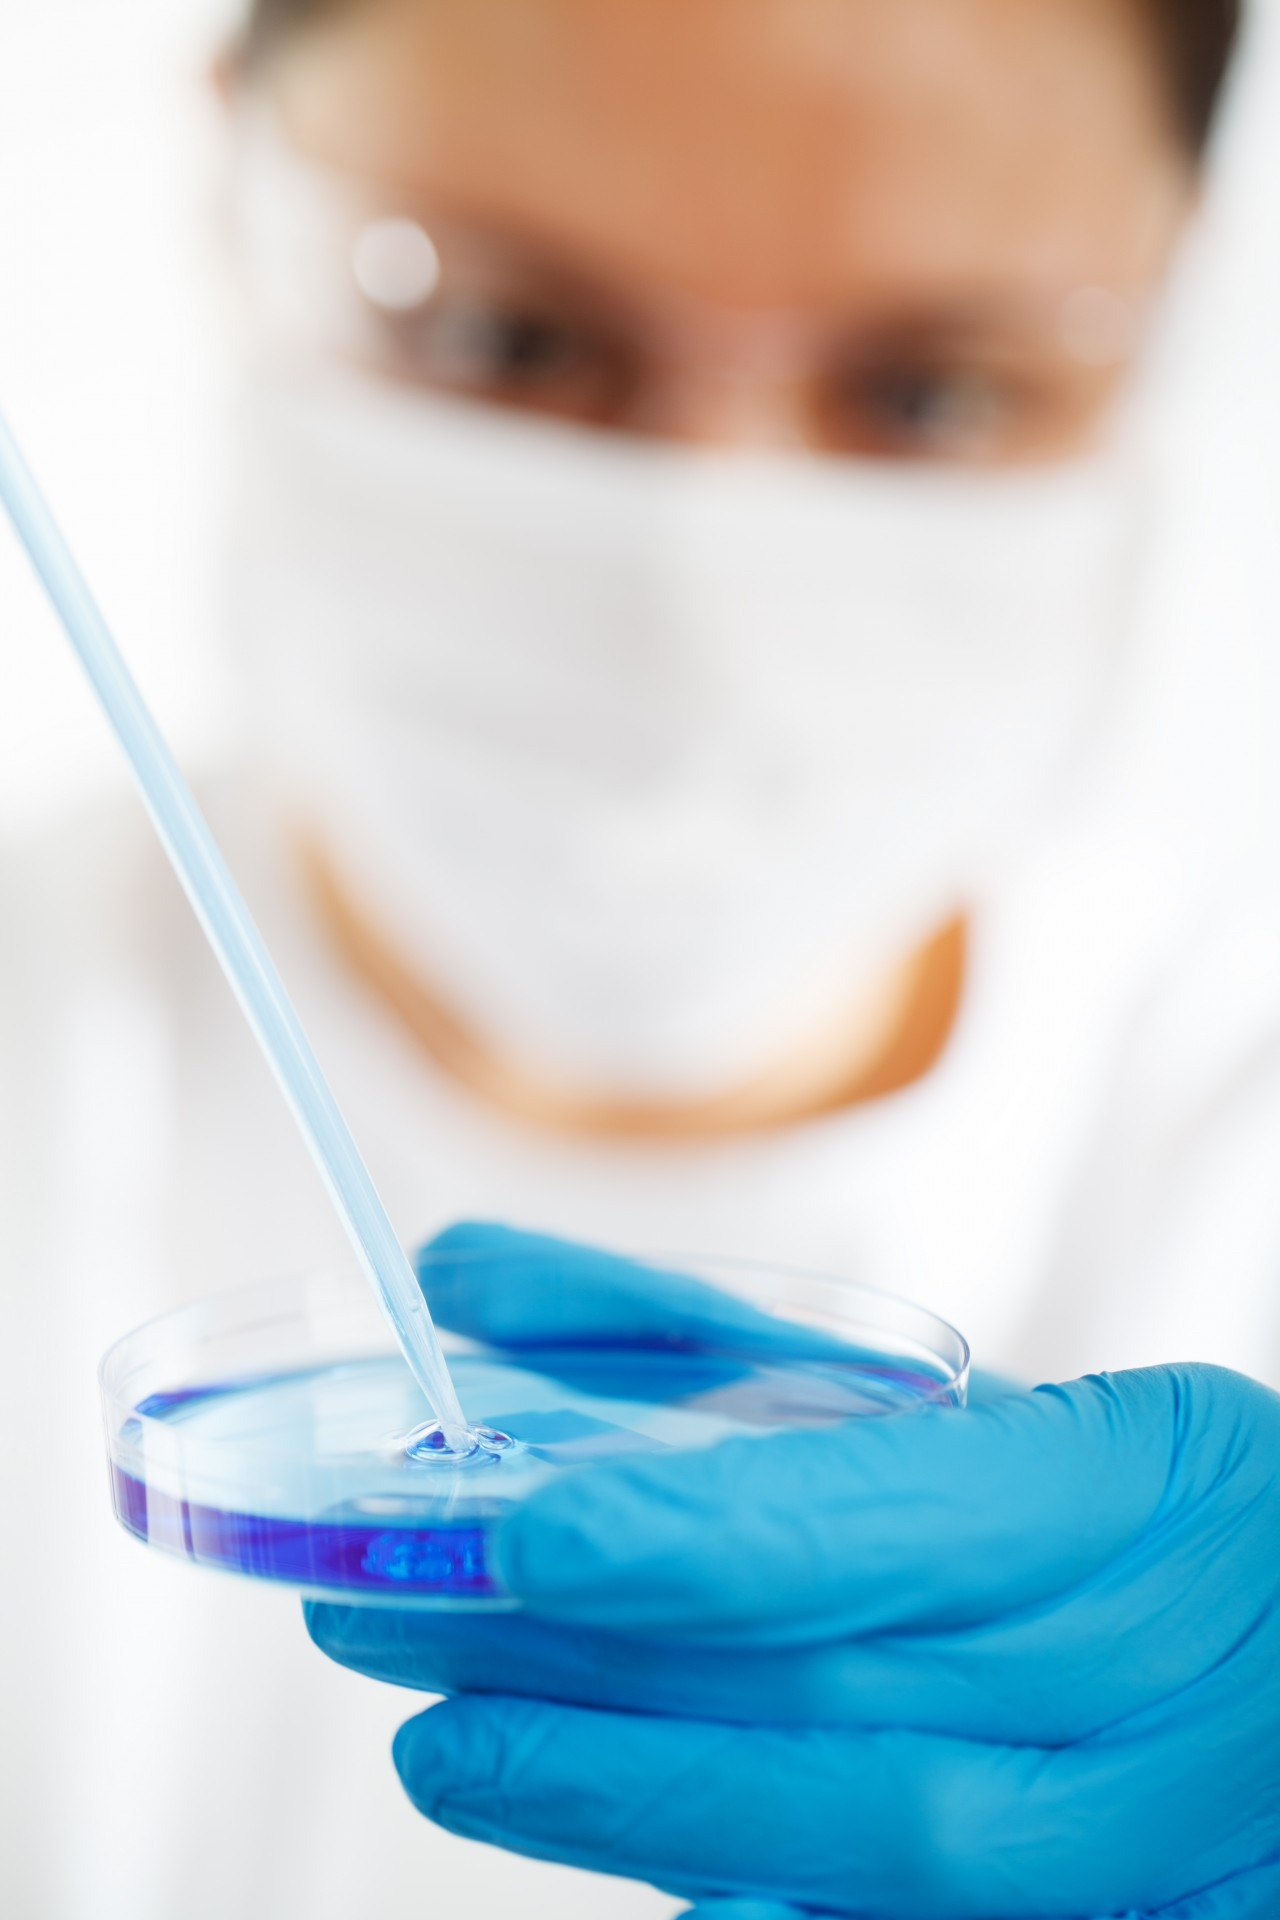
\includegraphics[scale=1]{capa}}} % Image background
	
	\AddToShipoutPicture*{\put(116,650){
\includegraphics[scale=.75]{brasao.png}}} % Image background
	
	\AddToShipoutPicture*{\put(244,200){
\includegraphics[scale=0.2]{ifgvertical}}} % Image background
	
	\vspace*{4.5cm}
	
	\centering
	\par
	{\Huge Projeto Pedagógico}\vspace*{1.5cm}
	\par
	\fontsize{40}{40}
	\selectfont
	Técnico Integrado em Tempo Integral em Biotecnologia\vspace*{10cm}
	\par
	{\Huge 2019}
	\par
\endgroup
\pagebreak

%----------------------------------------------------------------------------------------
%	PEOPLE PAGE
%----------------------------------------------------------------------------------------
\chapterimage{banner3} % Chapter heading image
\begin{center}
	\par
	{\large PRESIDENTE DA REPÚBLICA \\ Jair Messias Bolsonaro}\vspace*{1cm}
	\par
	{\large MINISTRO DA EDUCAÇÃO \\ Nome do Ministro}\vspace*{1cm}
	\par
	{\large SECRETÁRIO DE EDUCAÇÃO PROFISSIONAL E TECNOLÓGICA \\ Alexandro Ferreira de Souza}\vspace*{1cm}
	\par
	{\large REITOR DO INSTITUTO FEDERAL DE GOIÁS \\ Jerônimo Rodrigues da Silva}\vspace*{1cm}
	\par
	{\large PRÓ-REITOR DE PESQUISA E PÓS-GRADUAÇÃO \\ Ruberley Rodrigues de Souza}\vspace*{1cm}
	\par
	{\large DIRETORIA DE PÓS-GRADUAÇÃO \\ Clarinda Aparecida da Silva}\vspace*{1cm}
	\par
	{\large COORDENADOR DO CURSO \\ Waldeyr Mendes Cordeiro da Silva}\vspace*{1cm}
\end{center}

\chapterimage{banner3} % Chapter heading image
\renewcommand\contentsname{Sumário}
\tableofcontents

%----------------------------------------------------------------------------------------
%	CHAPTER
%----------------------------------------------------------------------------------------
\chapterimage{01.jpg} % Chapter heading image
\chapter{Apresentação}
\vspace{6em}
\begin{flushright}
	\textit{ }
\end{flushright}
\vspace{12em}

\todo[inline]{Texto...}


%-----------------------------------------------
\newpage  
%------------------------------------------------
\section{Identificação do Curso}
\begin{itemize}
	\item \textbf{Instituição Proponente:} Instituto Federal de Goiás
	\item \textbf{Nome do curso:} Técnico Integrado em Tempo Integral em Biotecnologia
	\item \textbf{Carga Horária do Curso:} 3802 horas
	\item \textbf{Forma de oferta:} Presencial
	\item \textbf{Duração:} 3 anos
	\item \textbf{Número de Vagas:} 30 vagas anuais
	\item \textbf{Local de Oferta:} Instituto Federal de Goiás - Câmpus Formosa
	\item \textbf{Reitor:} Jerônimo Rodrigues da Silva
	\item \textbf{Pró-Reitora de Ensino:} Oneida Cristina Gomes Barcelos Irigon
	\item \textbf{Pró-Reitor de Pesquisa, Pós-Graduação e Inovação:} Ruberley Rodrigues de Souza
	\item \textbf{Diretoria de Pós-Graduação:} Clarinda Aparecida da Silva
\end{itemize}

\section{Comissão Organizadora}
	\begin{itemize}[label=\bfseries]
		\item \nameref{AdrianoDarosci}
		\item ...
		\item \nameref{WaldeyrMendes}
	\end{itemize}

%----------------------------------------------------------------------------------------
%	CHAPTER
%----------------------------------------------------------------------------------------
\chapterimage{02.jpg} % Chapter heading image

\chapter{Introdução}
\vspace{6em}
\begin{flushright}
	\textit{\textcolor{white}{Foto: Adriano Darosci}}
\end{flushright}
\vspace{12em}

\todo[inline]{Texto...}

\section{Justificativa}

\todo[inline]{Texto...}

\section{Público Alvo}

\todo[inline]{Texto...}

\section{Objetivos}\label{objetivos}
\subsection{Objetivo Geral}

\todo[inline]{Texto...}

\subsection{Objetivos Específicos}
\begin{itemize}
\item Texto... 
\end{itemize}

\section{Requisitos para Acesso ao Curso}

\todo[inline]{Texto...}


\section{Perfil do Egresso}

O Técnico em Biotecnologia executa atividades laboratoriais de biotecnologia e biociências em centros de pesquisas, indústrias e empresas no setor de saúde humana e animal, ambiental e agropecuário. 
Opera, controla e monitora processos industriais e laboratoriais, incluindo laboratórios de saúde e ambiental. 
Prepara materiais, meios de cultura, soluções e reagentes. 
Analisa substâncias e materiais biológicos. 
Cultiva \textit{in vivo} e \textit{in vitro} microrganismos, células e tecidos animais e vegetais. 
Realiza o preparo de amostras dos tecidos animais e vegetais. 
Extrai, replica e quantifica biomoléculas.
Realiza a produção de imunobiológicos, vacinas, diluentes, kits de diagnóstico e bioprocessos industriais. 
Colabora nas atividades de perícia criminal e investigação genética. 
Desenvolve pesquisa de melhoramento genético. 
Opera a criação e manejo de animais de experimentação. 
Controla a qualidade e a compra de matérias-primas, insumos e produtos.

\subsection{Campo de atuação}

O campo de atuação inclui, mas não limita-se a empresas, indústrias, agroindústrias, instituições de pesquisa, ensino e desenvolvimento em biociências e produtos biotecnológicos.
Laboratórios de controle de qualidade de biomoléculas, de bioprocessos, de biologia molecular, de toxicologia, de biodiagnósticos e de análises clínicas. 
Bancos de materiais biológicos e de genes. 
Empresas de consultorias, assistência técnica, comercialização de insumos e equipamentos utilizados na área de biociências e biotecnologia. 
Indústrias alimentícias, de cosméticos, bebidas e farmacêutica. 
Laboratório de agropecuária e ambiental. 
Estações de monitoramento e tratamento biológicos da água. 
Escritórios de patentes biotecnológicas. 
Empreendimento próprio.

\subsection{Ocupações CBO associadas}

325305-Técnico em biotecnologia. 

325310-Técnico em imunobiológicos.

\subsection{Normas associadas ao exercício profissional}

Lei nº 11.105/2005. 

Decreto nº 5.591/2005. 

Decreto nº 5.950/2006. 

Decreto nº 6.925/2009. 

Decreto nº 5.705/2006. 

Decreto nº 6.041/2007.

\subsection{Possibilidades de verticalização para cursos de graduação no itinerário formativo}

Curso superior de tecnologia em biotecnologia. 
Curso superior de tecnologia em saneamento ambiental. 
Bacharelado em ciências biológicas. 
Bacharelado em biomedicina. 
Bacharelado em farmácia. 
Bacharelado em nutrição. 
Bacharelado em engenharia de alimentos. 
Bacharelado em engenharia química. 
Bacharelado em biotecnologia. 
Bacharelado em engenharia ambiental.

%----------------------------------------------------------------------------------------
%	CHAPTER
%----------------------------------------------------------------------------------------
\chapterimage{03.jpg} % Chapter heading image

\chapter{Organização do Curso}
\vspace{6em}
\begin{flushright}
	\textit{\textcolor{white}{``O homem, por ser inacabado, tende à perfeição. A educação é, portanto, um
			processo contínuo que só acaba com a morte'' (FURTER, 1973).}}
\end{flushright}
\vspace{12em}

\section{Forma de Oferta}\label{carga}

O Curso Técnico Integrado ao Ensino Médio em Biotecnologia funcionará em período matutino e vespertino, com oferta de 30 vagas anuais. 
O Curso tem duração total de~\VER{3802} horas, sendo \VER{3402} horas de disciplinas e \VER{200} horas de estágio curricular supervisionado e \VER{200} horas de atividades complementares.
A duração mínima é de 3 (três) anos e o prazo máximo de integralização dos cursos da educação profissional técnica de nível médio integrado ao ensino médio é do dobro do tempo da sua duração. 
Logo, o máximo será de 6 (seis) anos, em conformidade com a legislação vigente. 
Após o prazo previsto por lei o aluno terá que se submeter a novo processo seletivo, caso deseje concluí-lo.


\section{Matriz Curricular}\label{matriz}

As disciplinas estão organizadas em séries anuais, conforme a Tabela~\ref{tab:matriz}, com a seguinte perspectiva:
\begin{itemize}
	\item 1º Ano: Construção das bases científicas e epistemológicas; Desenvolvimento das competências previstas na Base Nacional Comum Curricular (BNCC);
	\item 2º Ano: Contextualização das bases científicas e epistemológicas; Desenvolvimento das competências previstas na Base Nacional Comum Curricular (BNCC); Desenvolvimento de competências primárias em Biotecnologia;
	\item 3º Ano: Consolidação e aplicação das bases científicas e epistemológicas; Desenvolvimento das competências previstas na Base Nacional Comum Curricular (BNCC); Desenvolvimento de competências profissionais em Biotecnologia;
\end{itemize}


\begin{table}[H]
	\centering
	\caption{Matriz Curricular do Curso Técnico em Biotecnologia Integrado ao Ensino Médio em Tempo Integral.}
	\label{tab:matriz}
	\resizebox{\textwidth}{!}{%
		\begin{tabular}{|l|l|l|l|l|l|}
			\hline
			Núcleo                         & Disciplinas                                      & 1º Ano     & 2º Ano    & 3º Ano    & CH Totais \\ \hline
			\multirow{12}{*}{Básico}       & \nameref{disc:artes}                             & 2          & 2         & 0         & 108       \\ \cline{2-6} 
			& \nameref{disc:ingles}                      & 4          & 0         & 0         & 108       \\ \cline{2-6} 
			& \nameref{disc:educacaofisica}                                  & 2          & 2         & 0         & 108       \\ \cline{2-6} 
			& \nameref{disc:linguaportuguesa}  & 4          & 4         & 4         & 324       \\ \cline{2-6} 
			& \nameref{disc:matematica}                        & 4          & 2         & 2         & 216       \\ \cline{2-6} 
			& \nameref{disc:geografia}                                        & 2          & 2         & 2         & 162       \\ \cline{2-6} 
			& \nameref{disc:historia}                                        & 2          & 2         & 2         & 162       \\ \cline{2-6} 
			& \nameref{disc:fisica}                                           & 2          & 2         & 2         & 162       \\ \cline{2-6} 
			& \nameref{disc:quimica}                                          & 4          & 0         & 0         & 108       \\ \cline{2-6} 
			& \nameref{disc:biologia}                                         & 4          & 0         & 0         & 108       \\ \cline{2-6} 
			& \nameref{disc:filosofia}                                        & 2          & 2         & 2         & 162       \\ \cline{2-6} 
			& \nameref{disc:sociologia}                                       & 2          & 2         & 2         & 162       \\ \hline
			\multicolumn{2}{|l|}{Carga horária semanal Núcleo Comum}                          & 34         & 20        & 16        & 1890      \\ \hline
			\multirow{7}{*}{Politécnico}   & Informática e propriedade intelectual            & 2          & 0         & 0         & 54        \\ \cline{2-6} 
			& \nameref{disc:espanhol_libras}          & 0          & 0         & 2         & 54        \\ \cline{2-6} 
			& \nameref{disc:fermentacao}                                      & 0          & 2         & 0         & 54        \\ \cline{2-6} 
			& \nameref{disc:bioquimica}                                       & 0          & 4         & 0         & 108       \\ \cline{2-6} 
			& \nameref{disc:microbiologia}                                    & 0          & 0         & 4         & 108       \\ \cline{2-6} 
			& \nameref{disc:biomol}                      & 0          & 4         & 0         & 108       \\ \cline{2-6} 
			& \nameref{disc:laboratorio}       & 2          & 0         & 0         & 54        \\ \hline
			\multicolumn{2}{|l|}{Carga horária semanal Núcleos Básico  e Politécnico}         & 38         & 30        & 22        & 2430      \\ \hline
			\multirow{6}{*}{Técnico}       & \nameref{disc:biotecAnimal}                             & 0          & 4         & 0         & 108       \\ \cline{2-6} 
			& \nameref{disc:biotecVegetal}                            & 0          & 4         & 0         & 108       \\ \cline{2-6} 
			& \nameref{disc:biotecAlimentos}                       & 0          & 0         & 4         & 108       \\ \cline{2-6} 
			& \nameref{disc:biotecFarmacos}        & 0          & 0         & 4         & 108       \\ \cline{2-6} 
			& \nameref{disc:biotecSaude}                    & 0          & 0         & 4         & 108       \\ \cline{2-6} 
			& \nameref{disc:producao}                          & 0          & 0         & 4         & 108       \\ \hline
			\multicolumn{2}{|l|}{Carga horária semanal Núcleos Básico, Politécnico e Técnico} & 38         & 38        & 38        & 3078      \\ \hline
			\multicolumn{2}{|l|}{\nameref{disc:estudo}}                                  & 4          & 4         & 4         & 324       \\ \hline
			\multicolumn{5}{|l|}{Estágio curricular}                                                                               & 200       \\ \hline
			\multicolumn{5}{|l|}{Atividades complementares}                                                                        & 200       \\ \hline
			\multicolumn{2}{|l|}{\multirow{2}{*}{Carga horária}}                              & \multicolumn{3}{l|}{Total Semanal} & Total     \\ \cline{3-6} 
			\multicolumn{2}{|l|}{}                                                            & 42         & 42        & 42        & 3802      \\ \hline
			Número de disciplinas por ano  &                                                  & 14         & 14        & 13        & 41        \\ \hline
		\end{tabular}%
	}
\end{table}

\section{Metodologia de Ensino-Aprendizagem}\label{metodologia}

\todo[inline]{Descrever a bordagem de Núcleo Politécnico, e curriculo integrado...}


\subsection{Trabalhos Discentes}\label{trabdiscentes}

\subsubsection{Atividades Não Presenciais}

Respeitados os mínimos previstos de duração e carga horária total, o plano de curso técnico de nível médio pode prever atividades não presenciais, até 20\% (vinte por cento) da carga horária diária do curso, desde que haja suporte tecnológico e seja garantido o atendimento por docentes e tutores~\cite{Resolucao06De2012}.

\subsubsection{Avaliação}

\todo[inline]{Utilizar a disciplina de debates semanais como 50\% da nota para todas as disciplinas?}

\section{Certificação}

Para obter o Certificado de Especialização em Ambiente, Ciência e Ensino do Cerrado, o discente deverá satisfazer as seguintes exigências:
\begin{itemize}
	\item Ser aprovado em todas as disciplinas do curso com nota mínima igual a 7,0 (sete) e freqüência igual ou superior a 75\% da carga horária da disciplina;
	\item Defender publicamente a monografia produzida perante uma Banca composta por, no mínimo, três professores (orientador, mais dois professores convidados, um externo e um interno ao campus IFG/Formosa) obtendo conceito Aprovado (AP);
	\item Possuir pelo menos um certificado que comprove a apresentação (pôster ou oral) de resultados relacionados à monografia exigida por essa pós-graduação em evento científico externo ao IFG (congressos, seminários, simpósios) cuja abrangência é, no mínimo, regional;
	\item Possuir documento (carta eletrônica ou impressa) que ateste a submissão em um periódico indexado de pelo menos um artigo produzido a partir dos resultados obtidos com o trabalho de conclusão de curso exigido por essa pós-graduação;
	\item Comprovar a quitação de suas obrigações junto à biblioteca do Campus Formosa do Instituto Federal de Educação, Ciência e Tecnologia de Goiás;
	\item Entregar toda a documentação exigida pelo processo seletivo.
\end{itemize}

O Certificado será emitido pelo Instituto Federal de Educação, Ciência e Tecnologia de Goiás, nos termos da Resolução CNE/CES n.º 1, de 8 de junho de 2007.	

%----------------------------------------------------------------------------------------
%	CHAPTER
%----------------------------------------------------------------------------------------
%------------------------------------------------
\chapterimage{04.jpg} % Chapter heading image

\chapter{Ementas}
\vspace{6em}
\begin{flushright}
	\textit{\textcolor{white}{Foto: Adriano Darosci}}
\end{flushright}
\vspace{12em}

\section{Ementas do Núcleo Básico}\label{ementasBasico}

\newpage
\section{Artes}\label{disc:artes}
\begin{itemize}
	\item \textbf{Carga horária (hora/aula):} 108
	\item \textbf{Docente Responsável:}
	\item \textbf{Conceitos-Chave:}
	\begin{itemize}
		\item NNNNN
		\item NNNNN
	\end{itemize}
	\item \textbf{Ementa:}Estudo sobre arte em suas linguagens, códigos e tecnologias específicas e suas influências culturais e educativas na sociedade;
	Conhecimento da arte como identidade, memória e criação, considerando suas expressões regionais e ressaltando as influências africanas e indígenas;
	Fundamentos, conceitos, funções, especificidades e características das artes visuais, dança, música, teatro e audiovisual;
	Abordagens histórico-reflexivas das produções artístico-culturais da humanidade;
	Projetos de investigação e experimentação artística com técnicas, materiais, estilos e gêneros variados;
	Apreciação e compreensão de diferentes poéticas em diálogo com as manifestações artísticas regionais nas diversas linguagens;
	Estudo das matrizes culturais da arte brasileira, em especial as africanas e indígenas, a partir das diversas visões e versões de seus representantes;
	Relações entre arte e mundo do trabalho;
	\item \textbf{Bibliografia básica}
	\begin{enumerate}
		\item NNNNN
	\end{enumerate}
	\item \textbf{Bibliografia complementar}
	\begin{enumerate}
		\item 
	\end{enumerate}	
\end{itemize}

\newpage
\section{Língua estrangeira - Inglês}\label{disc:ingles}
\begin{itemize}
	\item \textbf{Carga horária (hora/aula):} 108
	\item \textbf{Docente Responsável:}
	\item \textbf{Conceitos-Chave:}
	\begin{itemize}
		\item NNNNN
		\item NNNNN
	\end{itemize}
	\item \textbf{Ementa:} Leitura, compreensão e interpretação de textos orais e escritos, estabelecendo relações entre língua, cultura e sociedade;
	Estudo de elementos morfossintáticos, semânticos e fonológicos da língua inglesa;
	Desenvolvimento das habilidades comunicativas com ênfase na leitura;
	Leitura, compreensão e interpretação de textos escritos, ligados à área de conhecimento do curso;
	\item \textbf{Bibliografia básica}
	\begin{enumerate}
		\item NNNNN
	\end{enumerate}
	\item \textbf{Bibliografia complementar}
	\begin{enumerate}
		\item 
	\end{enumerate}	
\end{itemize}


\newpage
\section{Educação física}\label{disc:educacaofisica}
\begin{itemize}
	\item \textbf{Carga horária (hora/aula):} 108
	\item \textbf{Docente Responsável:}
	\item \textbf{Conceitos-Chave:}
	\begin{itemize}
		\item NNNNN
		\item NNNNN
	\end{itemize}
	\item \textbf{Ementa:} Introdução e ampliação ao estudo, vivência e reflexão crítica dos temas da cultura corporal de movimento, abordados pela Educação Física;
	Compreensão dos aspectos biológicos, históricos, psicológicos, sociais, filosóficos e culturais, e suas relações com o meio ambiente e a diversidade humana, em uma perspectiva omnilateral;
	Educação Física e suas relações com o mundo do trabalho, a saúde e o lazer;
	\item \textbf{Bibliografia básica}
	\begin{enumerate}
		\item NNNNN
	\end{enumerate}
	\item \textbf{Bibliografia complementar}
	\begin{enumerate}
		\item 
	\end{enumerate}	
\end{itemize}


\newpage
\section{Língua portuguesa, leitura e produção de textos}\label{disc:linguaportuguesa}
\begin{itemize}
	\item \textbf{Carga horária (hora/aula):} 324
	\item \textbf{Docente Responsável:}
	\item \textbf{Conceitos-Chave:}
	\begin{itemize}
		\item NNNNN
		\item NNNNN
	\end{itemize}
	\item \textbf{Ementa:} Práticas de leitura, compreensão, interpretação e produção de textos de diversos gêneros textuais
	Análise linguística: integração dos níveis morfossintático e discursivo;
	Literatura brasileira e seus aspectos estilísticos e culturais em diálogo com a cultura afro-brasileira e indígena;
	Usos da Língua em diferentes registros e níveis de formalidade;
	\item \textbf{Bibliografia básica}
	\begin{enumerate}
		\item NNNNN
	\end{enumerate}
	\item \textbf{Bibliografia complementar}
	\begin{enumerate}
		\item 
	\end{enumerate}	
\end{itemize}


\newpage
\section{Matemática e estatística}\label{disc:matematica}
\begin{itemize}
	\item \textbf{Carga horária (hora/aula):} 216
	\item \textbf{Docente Responsável:}
	\item \textbf{Conceitos-Chave:}
	\begin{itemize}
		\item NNNNN
		\item NNNNN
	\end{itemize}
	\item \textbf{Ementa:} Conjuntos;
	Funções: introdução, afim, quadrática, modular, exponencial e logarítmica;
	Progressão aritmética;
	Progressão geométrica;
	Trigonometria;
	Funções trigonométricas;
	Geometria plana e espacial;
	Sistemas lineares;
	Matrizes;
	Determinantes.
	Geometria analítica; 
	Equações polinomiais; 
	Números complexos; 
	Combinatória; 
	Noções de Estatística e Probabilidade;
	Conceitos básicos de Bioestatística, tais como: organização dos dados quantitativos;
	Medidas de tendência central e de dispersão; distribuições; formulação de testes de hipóteses; 
	Médias e correlações;
	Matemática financeira;
	\item \textbf{Bibliografia básica}
	\begin{enumerate}
		\item NNNNN
	\end{enumerate}
	\item \textbf{Bibliografia complementar}
	\begin{enumerate}
		\item 
	\end{enumerate}	
\end{itemize}


\newpage
\section{Geografia}\label{disc:geografia}
\begin{itemize}
	\item \textbf{Carga horária (hora/aula):} 162
	\item \textbf{Docente Responsável:}
	\item \textbf{Conceitos-Chave:}
	\begin{itemize}
		\item NNNNN
		\item NNNNN
	\end{itemize}
	\item \textbf{Ementa:} A contribuição da Geografia para compreensão da realidade/mundo;
	Formas de representação espacial;
	A dinâmica da natureza e as interfaces com a formação das paisagens;
	Apropriação da natureza pelo trabalho e a questão ambiental;
	Espacialização das relações capitalistas de produção e a sociedade em rede;
	O processo de urbanização e a questão campo/cidade;
	Dinâmica demográfica e as relações étnico-culturais mundiais;
	Regionalização do espaço mundial e as novas modalidades de exclusão;
	Território, conflitos e geopolítica mundial;
	Constituição do território brasileiro;
	Formação das identidades no Brasil; 
	Dinâmica da natureza e a paisagem brasileira;
	Desenvolvimento industrial e urbanização no Brasil;
	Ocupação produtiva e a agricultura no Brasil; 
	Dinâmica demográfica e relações étnico-culturais no Brasil;
	Geografia de Goiás;
	\item \textbf{Bibliografia básica}
	\begin{enumerate}
		\item NNNNN
	\end{enumerate}
	\item \textbf{Bibliografia complementar}
	\begin{enumerate}
		\item 
	\end{enumerate}	
\end{itemize}



\newpage
\section{História}\label{disc:historia}
\begin{itemize}
	\item \textbf{Carga horária (hora/aula):} 162
	\item \textbf{Docente Responsável:}
	\item \textbf{Conceitos-Chave:}
	\begin{itemize}
		\item NNNNN
		\item NNNNN
	\end{itemize}
	\item \textbf{Ementa:} Estudos históricos em relações entre trabalho, produção, tecnologia, ciência, meio ambiente, questões étnico-culturais, de gênero, memória e as articulações destes elementos no
	interior de cada formação social, articulando o global e o local, bem como suas implicações nas diversas realidades; 
	Análise de processos de transformações/permanências/ resistências/semelhanças e diferenças nas dimensões políticas, econômicas, sociais e culturais;
	Sociedades ágrafas, antigas e medievais;
	Construção do mundo moderno: Europa, Ásia, Áfricas, Américas;
	Processos revolucionários dos séculos XVIII e XIX; 
	Brasil Império;
	Construção do mundo contemporâneo: do imperialismo à globalização; 
	Brasil República;
	\item \textbf{Bibliografia básica}
	\begin{enumerate}
		\item NNNNN
	\end{enumerate}
	\item \textbf{Bibliografia complementar}
	\begin{enumerate}
		\item 
	\end{enumerate}	
\end{itemize}


\newpage
\section{Física}\label{disc:fisica}
\begin{itemize}
	\item \textbf{Carga horária (hora/aula):} 162
	\item \textbf{Docente Responsável:}
	\item \textbf{Conceitos-Chave:}
	\begin{itemize}
		\item NNNNN
		\item NNNNN
	\end{itemize}
	\item \textbf{Ementa:} Movimentos: variações e conservações;
	Calor, ambiente e uso de energia;
	Som, imagem e informação;
	Equipamentos elétricos e telecomunicações;
	Matéria e radiação;
	\item \textbf{Bibliografia básica}
	\begin{enumerate}
		\item NNNNN
	\end{enumerate}
	\item \textbf{Bibliografia complementar}
	\begin{enumerate}
		\item 
	\end{enumerate}	
\end{itemize}


\newpage
\section{Química}\label{disc:quimica}
\begin{itemize}
	\item \textbf{Carga horária (hora/aula):} 108
	\item \textbf{Docente Responsável:}
	\item \textbf{Conceitos-Chave:}
	\begin{itemize}
		\item NNNNN
		\item NNNNN
	\end{itemize}
	\item \textbf{Ementa:} Matéria, energia, transformações, substâncias;
	Leis ponderais;
	Modelos e estrutura atômica;
	Tabela periódica;
	Ligações e interações Químicas;
	Funções inorgânicas;
	Reações Químicas;
	Soluções e propriedades coligativas;
	Eletroquímica;
	Termoquímica;
	Cinética Química;
	Estequiometria;
	Noções de radioatividade;
	Introdução à química orgânica;
	Funções orgânicas: hidrocarbonetos, oxigenadas e nitrogenadas, e suas principais reações; 
	Isomeria;
	\item \textbf{Bibliografia básica}
	\begin{enumerate}
		\item NNNNN
	\end{enumerate}
	\item \textbf{Bibliografia complementar}
	\begin{enumerate}
		\item 
	\end{enumerate}	
\end{itemize}



\newpage
\section{Biologia}\label{disc:biologia}
\begin{itemize}
	\item \textbf{Carga horária (hora/aula):} 108
	\item \textbf{Docente Responsável:}
	\item \textbf{Conceitos-Chave:}
	\begin{itemize}
		\item NNNNN
		\item NNNNN
	\end{itemize}
	\item \textbf{Ementa:} Seres vivos: Classificação, organização e importância econômica e ambiental;
	Ciclos Biogeoquímicos; 
	Célula: teoria, padrões e componentes; 
	Divisão celular;
	Morfologia e fisiologia humana;
	Origem da vida; 
	Teorias e mecanismos evolutivos;
	Ecologia: Conceitos básicos, ecologia de população, comunidades e ecossistemas; 
	Poluição e sustentabilidade;
	
	\item \textbf{Bibliografia básica}
	\begin{enumerate}
		\item NNNNN
	\end{enumerate}
	\item \textbf{Bibliografia complementar}
	\begin{enumerate}
		\item 
	\end{enumerate}	
\end{itemize}



\newpage
\section{Filosofia}\label{disc:filosofia}
\begin{itemize}
	\item \textbf{Carga horária (hora/aula):} 162
	\item \textbf{Docente Responsável:}
	\item \textbf{Conceitos-Chave:}
	\begin{itemize}
		\item NNNNN
		\item NNNNN
	\end{itemize}
	\item \textbf{Ementa:} Introdução à filosofia e ao filosofar;
	Elementos conceituais da teoria do conhecimento, da ontologia e das estruturas do pensamento e da linguagem;
	Fundamentos, concepções e relações da ética e da política; 
	Valores, direitos humanos, liberdade e virtude;
	Estado, poder, soberania, ideologia e formas de governo;
	Fundamentos conceituais da ciência, da subjetividade e da estética;
	O significado e as implicações dos processos científicos e da técnica; 
	A crise da razão;
	A constituição;
	\item \textbf{Bibliografia básica}
	\begin{enumerate}
		\item NNNNN
	\end{enumerate}
	\item \textbf{Bibliografia complementar}
	\begin{enumerate}
		\item 
	\end{enumerate}	
\end{itemize}



\newpage
\section{Sociologia}\label{disc:sociologia}
\begin{itemize}
	\item \textbf{Carga horária (hora/aula):} 162
	\item \textbf{Docente Responsável:}
	\item \textbf{Conceitos-Chave:}
	\begin{itemize}
		\item NNNNN
		\item NNNNN
	\end{itemize}
	\item \textbf{Ementa:} A Sociologia como ciência e sua origem; 
	Indivíduo e sociedade; 
	Instituições sociais; 
	Correntes clássicas do pensamento sociológico; 
	Modernidade e capitalismo;
	Cultura, etnocentrismo, relativismo cultural e diversidade: relações étnico-raciais, gênero, geração, sexualidade;
	Educação e sociedade; 
	Desigualdades sociais; 
	Trabalho e organização produtiva; 
	Globalização e Mundialização do do capital; 
	Indústria cultural e consumo;
	Estado, ideologia e regimes políticos; 
	Sistemas de governo; 
	Movimentos sociais;
	Cidadania e participação social;
	Política;
	\item \textbf{Bibliografia básica}
	\begin{enumerate}
		\item NNNNN
	\end{enumerate}
	\item \textbf{Bibliografia complementar}
	\begin{enumerate}
		\item 
	\end{enumerate}	
\end{itemize}


\newpage
\section{Ementas do Núcleo Politécnico}\label{ementasPolitecnico}


\newpage
\section{Informática e propriedade intelectual}\label{disc:info}
\begin{itemize}
	\item \textbf{Carga horária (hora/aula):} 54
	\item \textbf{Docente Responsável:}
	\item \textbf{Conceitos-Chave:}
	\begin{itemize}
		\item NNNNN
		\item NNNNN
	\end{itemize}
	\item \textbf{Ementa:} Uso da Internet e Noções de segurança da informação;
	Produção de textos usando software;
	Produção de planilha eletrônica;
	Produção de apresentações usando software;
	Elaboração de projetos de pesquisa; 
	Estrutura do trabalho científico;
	Propriedade intelectual: conceitos e modalidades;
	Gestão da Propriedade Intelectual;
	Gestão da inovação e transferência de tecnologia;
	Prospecção tecnológica;
	Noções de empreendedorismo;
	\item \textbf{Bibliografia básica}
	\begin{enumerate}
		\item NNNNN
	\end{enumerate}
	\item \textbf{Bibliografia complementar}
	\begin{enumerate}
		\item 
	\end{enumerate}	
\end{itemize}

\newpage
\section{Língua estrangeira – Espanhol ou LIBRAS}\label{disc:espanhol_libras}
\begin{itemize}
	\item \textbf{Carga horária (hora/aula):} 54
	\item \textbf{Docente Responsável:}
	\item \textbf{Conceitos-Chave:}
	\begin{itemize}
		\item NNNNN
		\item NNNNN
	\end{itemize}
	\item \textbf{Ementa:} Estruturas básicas da Língua Espanhola em uma abordagem contrastiva com a Língua Portuguesa em seus aspectos lexicais, sintáticos, semânticos, pragmáticos, discursivos e interculturais; 
	Habilidades comunicativas de recepção e produção em vários gêneros textuais a partir das especificidades de cada curso;
	Aspectos histórico-culturais do surdo. Noções básicas da gramática da Língua Brasileira de Sinais (LIBRAS);
	Vocabulário básico da LIBRAS;
	Práticas de conversação em LIBRAS;		
	\item \textbf{Bibliografia básica}
	\begin{enumerate}
		\item NNNNN
	\end{enumerate}
	\item \textbf{Bibliografia complementar}
	\begin{enumerate}
		\item 
	\end{enumerate}	
\end{itemize}


\newpage
\section{Fermentação}\label{disc:fermentacao}
\begin{itemize}
	\item \textbf{Carga horária (hora/aula):} 54
	\item \textbf{Docente Responsável:}
	\item \textbf{Conceitos-Chave:}
	\begin{itemize}
		\item NNNNN
		\item NNNNN
	\end{itemize}
	\item \textbf{Ementa:} Fermentação industriais;
	Conceituação de processo fermentativo; 
	Microrganismos para utilização industrial; 
	Matérias primas e meios de fermentação para utilização industrial; 
	Principais etapas de um processo fermentativo; 
	Classificação dos processos fermentativos quanto ao desenvolvimento do agente, regime de condução do processo e necessidade de oxigênio;
	Produtos do metabolismo microbiano de interesse na indústria farmacêutica, de alimentos e afins; 
	Enzimologia industrial; 
	Cinética de crescimento microbiano;
	Esterilização de equipamentos, meios e ar;
	Biorreatores;
	Bioprocessos.;
	\item \textbf{Bibliografia básica}
	\begin{enumerate}
		\item NNNNN
	\end{enumerate}
	\item \textbf{Bibliografia complementar}
	\begin{enumerate}
		\item 
	\end{enumerate}	
\end{itemize}

\newpage
\section{Bioquímica}\label{disc:bioquimica}
\begin{itemize}
	\item \textbf{Carga horária (hora/aula):} 108
	\item \textbf{Docente Responsável:}
	\item \textbf{Conceitos-Chave:}
	\begin{itemize}
		\item NNNNN
		\item NNNNN
	\end{itemize}
	\item \textbf{Ementa:} Introdução à Bioquímica; 
	Biomoléculas e nutrientes;
	Reações de biossíntese e degradação;
	Metabolismo e aplicações de carboidratos, lipídios e proteínas;
	Seminários de bioquímica;
	\item \textbf{Bibliografia básica}
	\begin{enumerate}
		\item NNNNN
	\end{enumerate}
	\item \textbf{Bibliografia complementar}
	\begin{enumerate}
		\item 
	\end{enumerate}	
\end{itemize}

\newpage
\section{Microbiologia}\label{disc:microbiologia}
\begin{itemize}
	\item \textbf{Carga horária (hora/aula):} 108
	\item \textbf{Docente Responsável:}
	\item \textbf{Conceitos-Chave:}
	\begin{itemize}
		\item NNNNN
		\item NNNNN
	\end{itemize}
	\item \textbf{Ementa:} Introdução e histórico da microbiologia; 
	Microrganismos: classificação, citologia, morfologia, metabolismo, crescimento, controle do crescimento, genética e técnicas microbiológicas;
	Microbiologia industrial; 
	Principais microrganismos e bioprodutos industriais: produção, melhoramento e características gerais;
	
	\item \textbf{Bibliografia básica}
	\begin{enumerate}
		\item NNNNN
	\end{enumerate}
	\item \textbf{Bibliografia complementar}
	\begin{enumerate}
		\item 
	\end{enumerate}	
\end{itemize}

\newpage
\section{Biologia Molecular e ômicas}\label{disc:biomol}
\begin{itemize}
	\item \textbf{Carga horária (hora/aula):} 108
	\item \textbf{Docente Responsável:}
	\item \textbf{Conceitos-Chave:}
	\begin{itemize}
		\item NNNNN
		\item NNNNN
	\end{itemize}
	\item \textbf{Ementa:} Dogma central da Biologia Molecular e o fluxo da informação genética;
	Estrutura, propriedades e características de ácidos nucléicos (DNA e RNA);
	Código genético; 
	Replicação e transcrição e tradução em procariotos e eucariotos;
	Mecanismo de processamento do mRNA eucariótico; 
	Histonas e empacotamento do DNA eucariótico; 
	Biossíntese de proteínas; 
	Amplificação gênica in vivo e in vitro; 
	Reparo e mutagênese;
	Técnicas básicas de manipulação genética;
	Genômica;
	Transcritômica;
	Metabolômica;
	Bioinformática básica;
	\item \textbf{Bibliografia básica}
	\begin{enumerate}
		\item NNNNN
	\end{enumerate}
	\item \textbf{Bibliografia complementar}
	\begin{enumerate}
		\item 
	\end{enumerate}	
\end{itemize}

\newpage
\section{Fundamentos de laboratório e biossegurança}\label{disc:laboratorio}
\begin{itemize}
	\item \textbf{Carga horária (hora/aula):} 54
	\item \textbf{Docente Responsável:}
	\item \textbf{Conceitos-Chave:}
	\begin{itemize}
		\item NNNNN
		\item NNNNN
	\end{itemize}
	\item \textbf{Ementa:} Princípios e teorias da bioética;
	Exercício profissional em biotecnologia; 
	O papel e os limites das ciências e do cientista; 
	Relações emergentes e persistentes da sociedade; 
	Bioética e a saúde pública, eutanásia e distanásia, segurança alimentar; transgênicos; 
	Especismo; 
	Tecnologias de ponta, bioterrorismo; 
	Aborto; 
	Patentes; 
	Direitos humanos;
	\item \textbf{Bibliografia básica}
	\begin{enumerate}
		\item NNNNN
	\end{enumerate}
	\item \textbf{Bibliografia complementar}
	\begin{enumerate}
		\item 
	\end{enumerate}	
\end{itemize}


\newpage
\section{Ementas do Núcleo Técnico}\label{ementasTecnico}


\newpage
\section{Biotecnologia animal}\label{disc:biotecAnimal}
\begin{itemize}
	\item \textbf{Carga horária (hora/aula):} 108
	\item \textbf{Docente Responsável:}
	\item \textbf{Conceitos-Chave:}
	\begin{itemize}
		\item NNNNN
		\item NNNNN
	\end{itemize}
	\item \textbf{Ementa:} 
	\item \textbf{Bibliografia básica}
	\begin{enumerate}
		\item NNNNN
	\end{enumerate}
	\item \textbf{Bibliografia complementar}
	\begin{enumerate}
		\item 
	\end{enumerate}	
\end{itemize}


\newpage
\section{Biotecnologia vegetal}\label{disc:biotecVegetal}
\begin{itemize}
	\item \textbf{Carga horária (hora/aula):} 108
	\item \textbf{Docente Responsável:}
	\item \textbf{Conceitos-Chave:}
	\begin{itemize}
		\item NNNNN
		\item NNNNN
	\end{itemize}
	\item \textbf{Ementa:} 
	\item \textbf{Bibliografia básica}
	\begin{enumerate}
		\item NNNNN
	\end{enumerate}
	\item \textbf{Bibliografia complementar}
	\begin{enumerate}
		\item 
	\end{enumerate}	
\end{itemize}


\newpage
\section{Biotecnologia de alimentos}\label{disc:biotecAlimentos}
\begin{itemize}
	\item \textbf{Carga horária (hora/aula):} 108
	\item \textbf{Docente Responsável:}
	\item \textbf{Conceitos-Chave:}
	\begin{itemize}
		\item NNNNN
		\item NNNNN
	\end{itemize}
	\item \textbf{Ementa:} 
	\item \textbf{Bibliografia básica}
	\begin{enumerate}
		\item NNNNN
	\end{enumerate}
	\item \textbf{Bibliografia complementar}
	\begin{enumerate}
		\item 
	\end{enumerate}	
\end{itemize}


\newpage
\section{Biotecnologia de fármacos e biodefensivos}\label{disc:biotecFarmacos}
\begin{itemize}
	\item \textbf{Carga horária (hora/aula):} 108
	\item \textbf{Docente Responsável:}
	\item \textbf{Conceitos-Chave:}
	\begin{itemize}
		\item NNNNN
		\item NNNNN
	\end{itemize}
	\item \textbf{Ementa:} 
	\item \textbf{Bibliografia básica}
	\begin{enumerate}
		\item NNNNN
	\end{enumerate}
	\item \textbf{Bibliografia complementar}
	\begin{enumerate}
		\item 
	\end{enumerate}	
\end{itemize}


\newpage
\section{Biotecnologia humana e saúde}\label{disc:biotecSaude}
\begin{itemize}
	\item \textbf{Carga horária (hora/aula):} 108
	\item \textbf{Docente Responsável:}
	\item \textbf{Conceitos-Chave:}
	\begin{itemize}
		\item NNNNN
		\item NNNNN
	\end{itemize}
	\item \textbf{Ementa:} 
	\item \textbf{Bibliografia básica}
	\begin{enumerate}
		\item NNNNN
	\end{enumerate}
	\item \textbf{Bibliografia complementar}
	\begin{enumerate}
		\item 
	\end{enumerate}	
\end{itemize}


\newpage
\section{Produção de bioprodutos}\label{disc:producao}
\begin{itemize}
	\item \textbf{Carga horária (hora/aula):} 108
	\item \textbf{Docente Responsável:}
	\item \textbf{Conceitos-Chave:}
	\begin{itemize}
		\item NNNNN
		\item NNNNN
	\end{itemize}
	\item \textbf{Ementa:} 
	\item \textbf{Bibliografia básica}
	\begin{enumerate}
		\item NNNNN
	\end{enumerate}
	\item \textbf{Bibliografia complementar}
	\begin{enumerate}
		\item 
	\end{enumerate}	
\end{itemize}



\newpage
\section{Estudo orientado e debates}\label{ementasEstudo}


\newpage
\section{Estudo orientado e debates}\label{disc:estudo}
\begin{itemize}
	\item \textbf{Carga horária (hora/aula):} 324
	\item \textbf{Docente Responsável:}
	\item \textbf{Conceitos-Chave:}
	\begin{itemize}
		\item NNNNN
		\item NNNNN
	\end{itemize}
	\item \textbf{Ementa:} Momento presencial com carga horária de 8 horas por semana para estudos dirigidos interdisciplinares; Debates de temas com dois grupos: um pró e um contra;
	\item \textbf{Bibliografia básica}
	\begin{enumerate}
		\item NNNNN
	\end{enumerate}
	\item \textbf{Bibliografia complementar}
	\begin{enumerate}
		\item 
	\end{enumerate}	
\end{itemize}


%----------------------------------------------------------------------------------------
%	CHAPTER X
%----------------------------------------------------------------------------------------
%------------------------------------------------
\chapterimage{05.jpg} % Chapter heading image

\chapter{Estrutura Física}
\vspace{6em}
\begin{flushright}
	\textit{\textcolor{white}{Foto: Adriano Darosci}}
\end{flushright}
\vspace{12em}

\section{Laboratório de Fisiologia Vegetal}

Equipado com: estufa de secagem, 3 estereoscópios, 3 microscópicos, geladeira, bancadas, 28 cadeiras, quadro e acervo didático (frutos, sementes e folhas herborizadas). 

\section{Laboratório de Bioqímica}

Equipado com: Balanças analítica e semi-analítica, chapas de aquecimento (com agitação magnética), analisador bioquímico, capela de fluxo laminar, agitadores de tubo de ensaio, banho-maria, bomba de vácuo, autoclave, estufas, destilador e deionizador de água e outros.

\section{Laboratório de Anatomia e Zoologia}

Equipado com: Bonecos anatômicos (de abdome) completos, conjuntos anatômicos artificiais de sistemas reprodutores femininos e masculinos, esqueletos completos (artificiais), amostras de animais (do cerrado e de outros biomas) conservados em frascos para visualização, animais empalhados, algumas peças anatômicas naturais de animais, lupas, microscópios, material para coleta de animais e saídas de campo, materiais e reagentes para o empalhamento de animais e outros.

\section{Laboratório de Microscopia e Microbiologia}

Equipado com:  25 microscópios e material para produção de lâminas (lâminas de corte, lâminas e lamínulas de vidro, corantes, fixadores, etc); Lupas, coleções de laminários e outros.

\section{Laboratório de Físico-Química}

Equipado com: pHmetros, destilador, capela de exaustão, estufa, banho-maria, balanças analítica e semi-analítica, deionizador, reator, aparelho de ponto de fusão,  e outros.

\section{Laboratório de Águas Residuais}

Equipado com: Condutivímetros, muflas, banho - maria, bomba de vácuo, analisador de oxigênio dissolvido, turbdímetro, estufa, balança, phmetro, destilador e outros.

\section{Laboratório de Ensino}

Espaço acadêmico voltado ao desenvolvimento e disseminação de tecnologias educacionais voltadas ao ensino de Ciências e Biologia.  Equipado com: acervo didático constituído por jogos, maquetes e representações físicas de organismos e processos biológicos.

\section{Laboratório de Física e Matemática}

O Laboratório de Física possui diversos equipamentos que contribui para o desenvolvimento das atividades experimentais nas áreas de mecânica, óptica, hidrostática, termologia e eletricidade.


\section{Laboratórios de Informática}

Dois laboratórios de informática com capacidade para até 30 estudantes, com acesso à Internet, computadores com sistema operacional Linux, softwares diversos.


\section{Biblioteca}

Biblioteca equipada com áreas de estudo individual e coletivo, 6 computadores com acesso ao portal de periódicos e acervo cerca de 7 mil exemplares, entre livros, livros em braile, cds, dvds e mapas;

\section{Teatro}

Teatro equipado com som e iluminação específica e acomodações para 320 pessoas sentadas;

\section{Outros Espaços}

3 salas para estudos coletivos e reuniões equipadas com mesas, cadeiras e televisor.


%----------------------------------------------------------------------------------------
%	CHAPTER X
%----------------------------------------------------------------------------------------
%------------------------------------------------
\chapterimage{06.jpg} % Chapter heading image
\chapter{Corpo Docente}
\vspace{6em}
\begin{flushright}
	\textit{\textcolor{white}{Foto: Adriano Darosci}}
\end{flushright}
\vspace{12em}

\section{Adriano Antonio Brito Darosci}\label{AdrianoDarosci}
\begin{itemize}
	\item Formação Básica: Ciências Biológicas
	\item Titulação Máxima: Doutor em Botânica
	\item Regime de Trabalho: Deicação Exclusiva
	\item 
\includegraphics[scale=.03]{Pictures/lattes}~\href{http://lattes.cnpq.br/4539795481921184}{Lattes: http://lattes.cnpq.br/4539795481921184}
\end{itemize}


\section{Anderson dos Anjos Pereira Pena}\label{AndersonPena}
\begin{itemize}
	\item Formação Básica: Pedagogia
	\item Titulação Máxima: Mestre em Cultura, Memória e Desenvolvimento Regional
	\item Regime de Trabalho: Dedicação Exclusiva
	\item 
\includegraphics[scale=.03]{Pictures/lattes}~\href{http://lattes.cnpq.br/9188378802285261}{Lattes: http://lattes.cnpq.br/9188378802285261}
\end{itemize}

\section{Ariane Bocaletto Frare}\label{ArianeFrare}
\begin{itemize}
	\item Formação Básica: Ciências Biológicas
	\item Titulação Máxima: Mestre em Genética
	\item Regime de Trabalho: Dedicação Exclusiva
	\item 
\includegraphics[scale=.03]{Pictures/lattes}~\href{http://lattes.cnpq.br/9984435027737343}{Lattes: http://lattes.cnpq.br/9984435027737343}
\end{itemize}


\section{Daniela Pereira Versieux}\label{DanielaVersieux}
\begin{itemize}
	\item Formação Básica: Ciências Biológicas
	\item Titulação Máxima: Mestre em Educação Tecnológica
	\item Regime de Trabalho: Dedicação Exclusiva
	\item 
\includegraphics[scale=.03]{Pictures/lattes}~\href{http://lattes.cnpq.br/9970651709122352}{Lattes: http://lattes.cnpq.br/9970651709122352}
\end{itemize}

\section{Fernanda Melo Duarte}\label{FernandaDuarte}
\begin{itemize}
	\item Formação Básica: Ciências Biológicas
	\item Titulação Máxima: Mestre em Genética
	\item Regime de Trabalho: Dedicação Exclusiva
	\item 
\includegraphics[scale=.03]{Pictures/lattes}~\href{http://lattes.cnpq.br/5338539796531801}{Lattes: http://lattes.cnpq.br/5338539796531801}
\end{itemize}

\section{Haissa Melo de Lima Gunther}\label{HaissaGunther}
\begin{itemize}
	\item Formação Básica: Ciências Biológicas
	\item Titulação Máxima: Mestre em Desenvolvimento Regional e Meio Ambiente
	\item Regime de Trabalho: Dedicação Exclusiva
	\item 
\includegraphics[scale=.03]{Pictures/lattes}~\href{http://lattes.cnpq.br/8481012955941397}{Lattes: http://lattes.cnpq.br/8481012955941397}
\end{itemize}

\section{Leandro Santos Goulart}\label{LeandroGoulart}
\begin{itemize}
	\item Formação Básica: Ciências Biológicas
	\item Titulação Máxima: Mestre em Biologia Animal
	\item Regime de Trabalho: Dedicação Exclusiva
	\item 
\includegraphics[scale=.03]{Pictures/lattes}~\href{http://lattes.cnpq.br/1871654436997150}{Lattes: http://lattes.cnpq.br/1871654436997150}
\end{itemize}

\section{Lemuel da Cruz Gandara}\label{LemuelGandara}
\begin{itemize}
	\item Formação Básica: Língua portuguesa e Estudos literários
	\item Titulação Máxima: Doutor em Literatura
	\item Regime de Trabalho: Dedicação Exclusiva
	\item 
\includegraphics[scale=.03]{Pictures/lattes}~\href{http://lattes.cnpq.br/7649361942295698}{Lattes: http://lattes.cnpq.br/7649361942295698}
\end{itemize}

\section{Marcos Augusto Schliewe}\label{MarcosSchliewe}
\begin{itemize}
	\item Formação Básica: Ciências Biológicas
	\item Titulação Máxima: Doutor em Botânica
	\item Regime de Trabalho: Dedicação Exclusiva
	\item 
\includegraphics[scale=.03]{Pictures/lattes}~\href{http://lattes.cnpq.br/8055970128960356}{Lattes: http://lattes.cnpq.br/8055970128960356}
\end{itemize}

\section{Patricia de Castilhos}\label{PatriciaCastilhos}
\begin{itemize}
	\item Formação Básica: Ciências Biológicas
	\item Titulação Máxima: Doutora em Imunologia e Parasitologia Aplicadas
	\item Regime de Trabalho: Dedicação Exclusiva
	\item 
\includegraphics[scale=.03]{Pictures/lattes}~\href{http://lattes.cnpq.br/7391339023174244}{Lattes: http://lattes.cnpq.br/7391339023174244}
\end{itemize}

\section{Thaís Amaral e Sousa}\label{ThaísSousa}
\begin{itemize}
	\item Formação Básica: Ciências Biológicas
	\item Titulação Máxima: Doutora em Ciências Biológicas
	\item Regime de Trabalho: Dedicação Exclusiva
	\item 
\includegraphics[scale=.03]{Pictures/lattes}~\href{http://lattes.cnpq.br/5246897777497752}{Lattes: http://lattes.cnpq.br/5246897777497752}
\end{itemize}

\section{Vinicius Sousa Ferreira}\label{ViniciusFerreira}
\begin{itemize}
	\item Formação Básica: Química, Farmácia e Bioquímica
	\item Titulação Máxima: Doutor em Química
	\item Regime de Trabalho: Dedicação Exclusiva
	\item 
\includegraphics[scale=.03]{Pictures/lattes}~\href{http://lattes.cnpq.br/6567799449480628}{Lattes: http://lattes.cnpq.br/6567799449480628}
\end{itemize}

\section{Waldeyr Mendes Cordeiro da Silva}\label{WaldeyrMendes}
\begin{itemize}
	\item Formação Básica: Sistemas de Informação e Ciências Biológicas
	\item Titulação Máxima: Doutor em Ciências Biológicas
	\item Regime de Trabalho: Dedicação Exclusiva
	\item 
\includegraphics[scale=.03]{Pictures/lattes}~\href{http://lattes.cnpq.br/2391349697609978}{Lattes: http://lattes.cnpq.br/2391349697609978}
	\item 
\includegraphics[scale=.15]{Pictures/orcid}~\href{https://orcid.org/0000-0002-8660-6331}{ORCID: https://orcid.org/0000-0002-8660-6331}
\end{itemize}
%----------------------------------------------------------------------------------------
%	CHAPTER X
%----------------------------------------------------------------------------------------
%------------------------------------------------
\chapterimage{Hypsiboas.jpg} % Chapter heading image
\chapter*{Conheça o IFG}
\vspace{6em}
\begin{flushright}
	\textit{\textcolor{white}{Foto: Adriano Darosci}}
\end{flushright}
\vspace{12em}

\section{Contato}

Instituto Federal de Educação, Ciência e Tecnologia de Goiás - Câmpus Formosa\\
Site:~\url{http://ifg.edu.br}\\
Endereço: XXXXX\\
Telefone: XXXXX \\
Twitter:XXXXXX \\
E-mails: XXXXXXX





% ----------------------------------------------------------------------------------------
% 	BIBLIOGRAPHY
% ----------------------------------------------------------------------------------------
%----------------------------------------------------------------------------------------
%	CHAPTER X
%----------------------------------------------------------------------------------------
%------------------------------------------------
\chapterimage{RoureaInduta.jpg} % Chapter heading image
%\chapter*{Referências Bibliográficas}
%\bibliography{bibliography}
%\renewcommand\bibname{Referências Bibliográficas}

\chapter*{Referências Bibliográficas}
\vspace{6em}
\begin{flushright}
	\textit{\textcolor{white}{Foto: Adriano Darosci}}
\end{flushright}
\vspace{12em}
%\addcontentsline{toc}{chapter}{\textcolor{verde}{Bibliography}}
%\section{Books}
%\addcontentsline{toc}{section}{Books}
%\printbibliography[heading=bibempty,type=book]
%\section{Articles}
%\addcontentsline{toc}{section}{Articles}
%\printbibliography[heading=bibempty,type=article]
\printbibliography[heading=bibempty]


%----------------------------------------------------------------------------------------

%----------------------------------------------------------------------------------------
%	INDEX
%----------------------------------------------------------------------------------------
%
%\cleardoublepage
%\phantomsection
%\setlength{\columnsep}{0.75cm}
%\addcontentsline{toc}{chapter}{\textcolor{verde}{Index}}
%\printindex


\end{document}